\chapter{Introdução}

A robótica é um ramo da tecnologia que lida com a concepção, construção,
operação e aplicação de máquinas capazes de realizar uma série de ações de
maneira autônoma.  Atualmente é um tópico em rápida ascensão.  Pesquisar,
projetar e fabricar novos robôs serve vários propósitos práticos tais como
domésticos, comerciais e militares.  Um dos problemas atuas da robótica é o
planejamento em ambientes multi-agentes dinâmicos e competitivos.  Um exemplo de
um problema dessa classe é um jogo de futebol de robôs, onde um grupo de robôs é
controlado por uma IA independente.  A Figura~\ref{fig:robocup2013} mostra uma
imagem da RoboCup 2013, competição internacional de robótica, onde a equipe
RoboIME (de alunos do Laboratório de Robótica do IME) participou.

\begin{figure}[h]
  \centering
  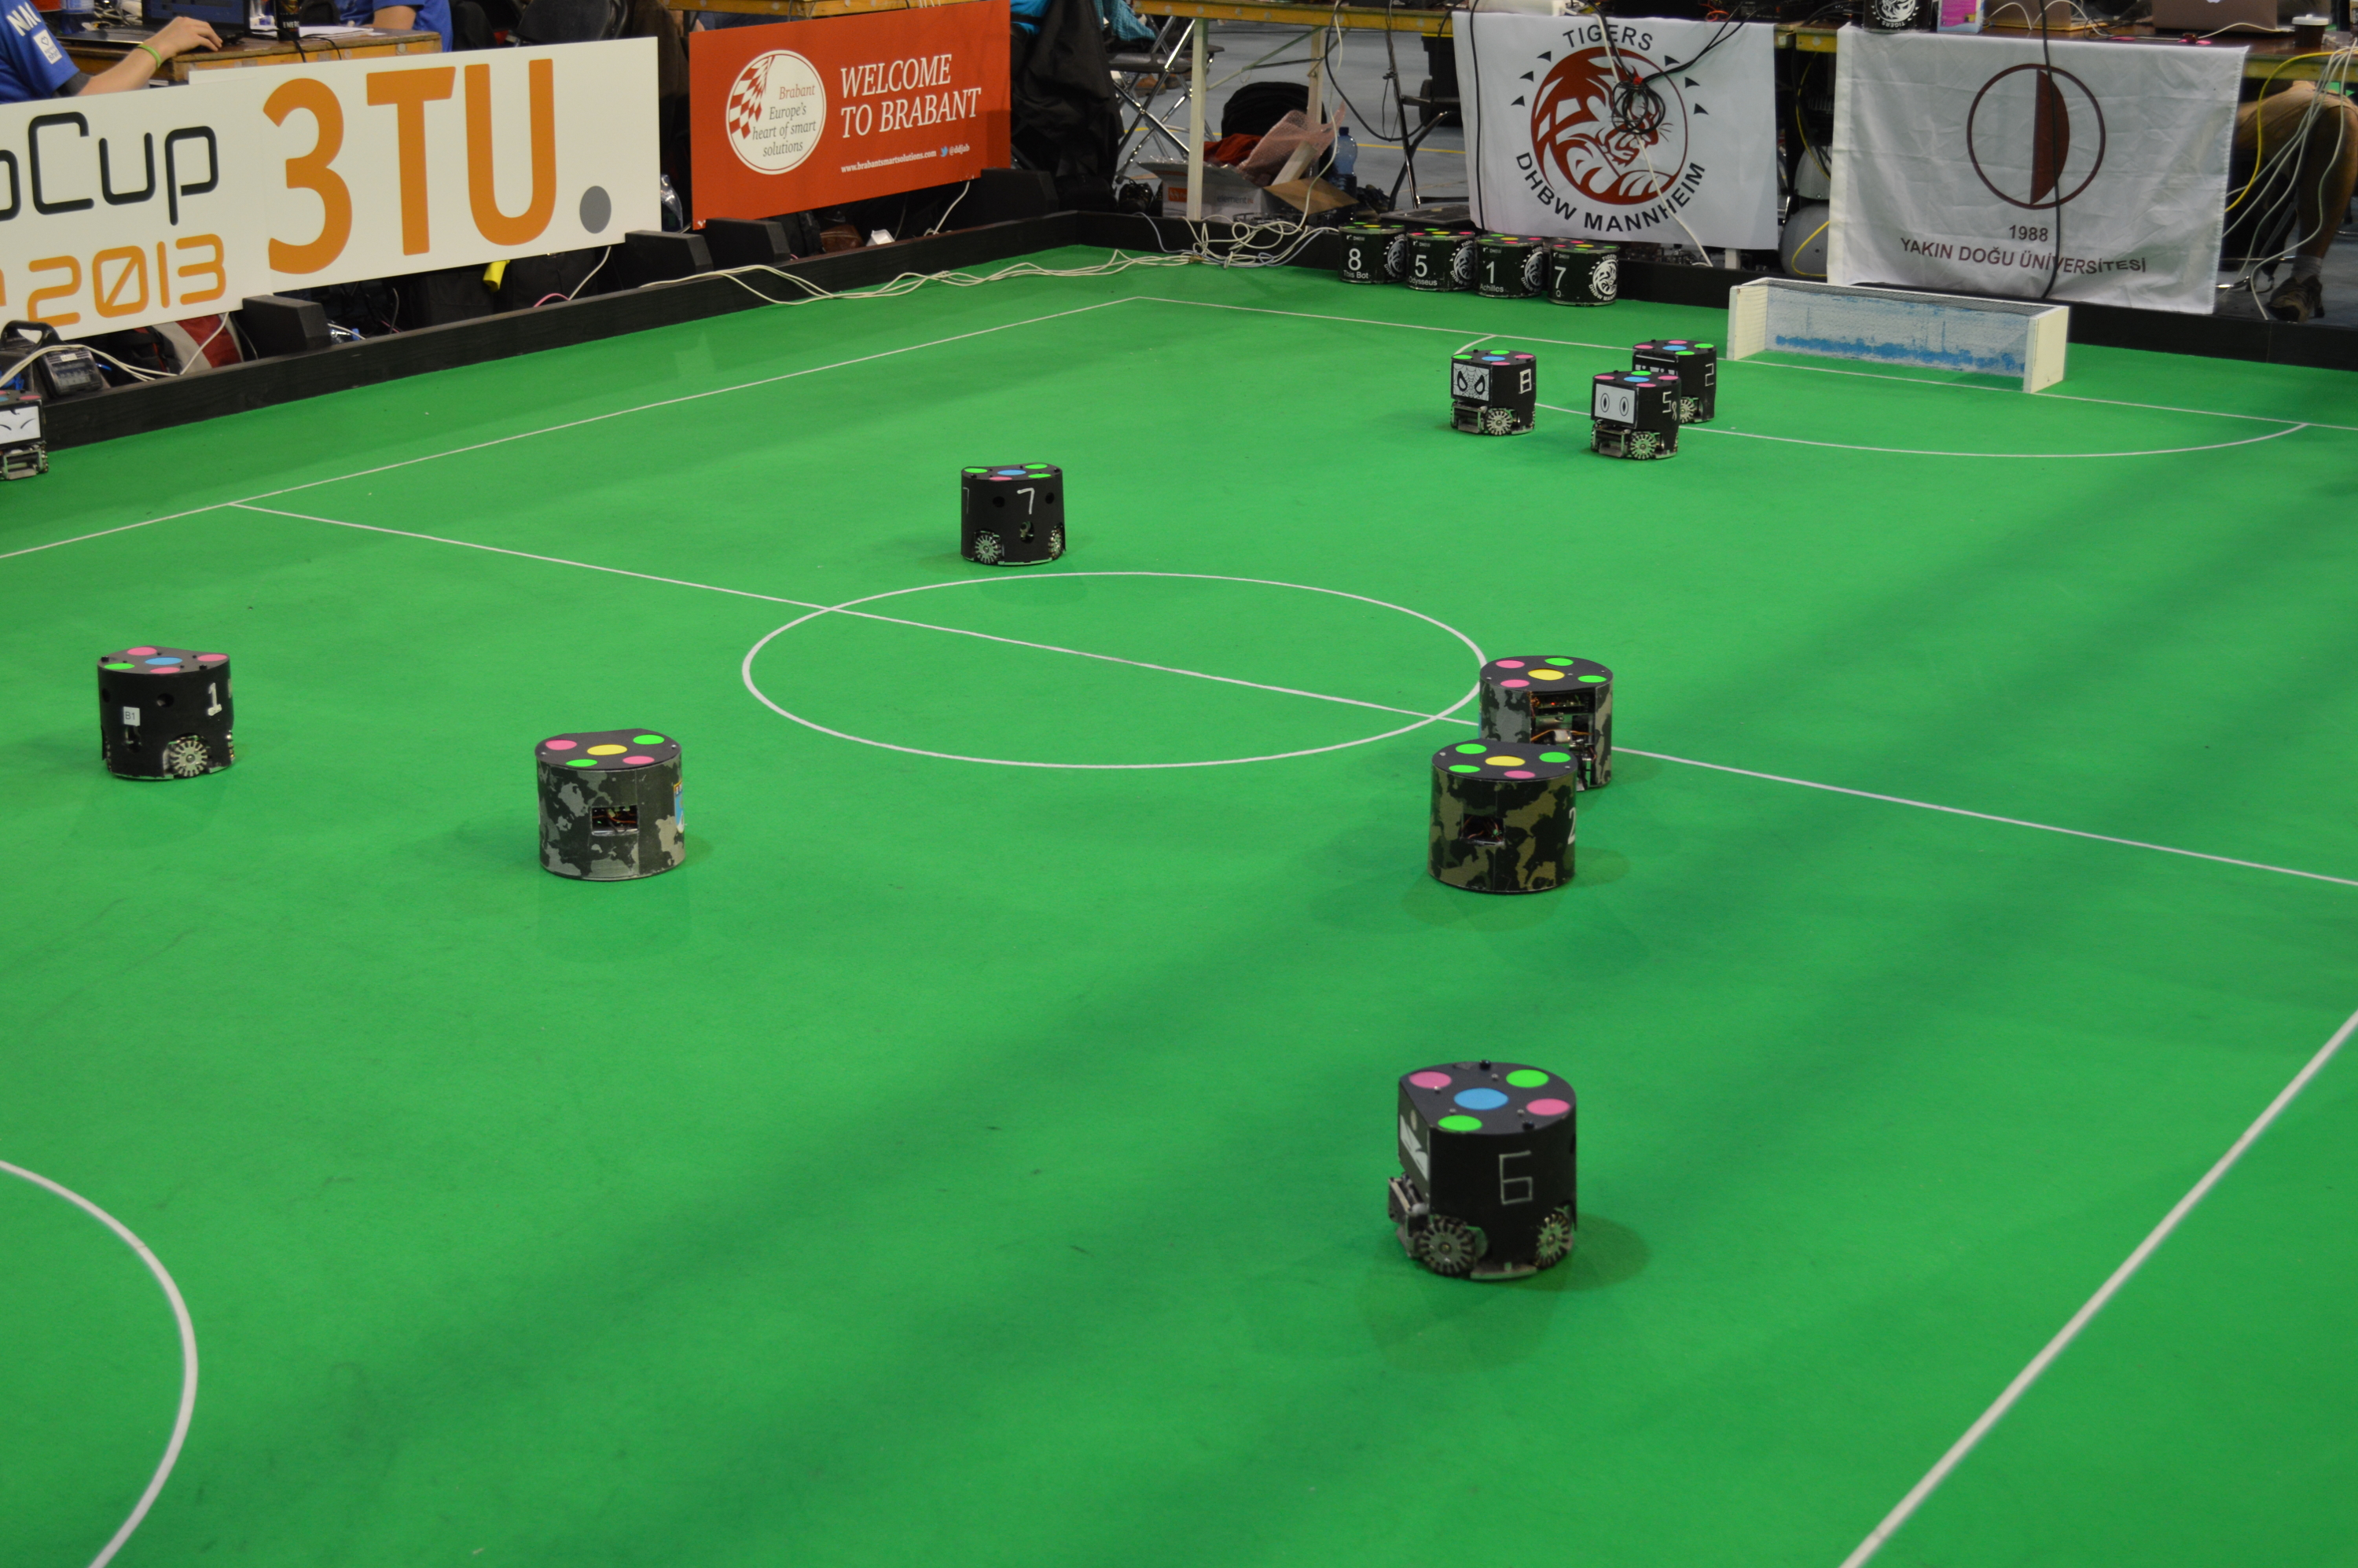
\includegraphics[width=0.8\linewidth]{robocup2013}
  \caption{Imagem da SSL \textit{RoboCup} 2013 em Eindhoven, na Holanda}\label{fig:robocup2013}
\end{figure}

Devido a alta complexidade desses ambientes, não é viável o planejamento
considerando diretamente as leis físicas.  Como consequência, limita-se as ações
possíveis do robô no modelo utilizado no planejamento para que se possa simular
mais situações em tempo hábil, uma vez que o ambiente está continuamente sujeito
a modificações.  Entretanto, para que as simulações sejam válidas, o robô real
deve estar em sintonia com seu modelo.  Com efeito, o robô real deve executar os
comandos conforme o robô simulado, caso o mesmo ambiente simulado seja
encontrado na prática.

A ideia de robôs jogando futebol foi mencionada pela primeira vez pelo professor
Alan Mackworth (University of British Columbia, Canadá) em um artigo intitulado
"On Seeing Robots", apresentado no Vision Interface 92 e posteriormente
publicado em um livro chamado Computer Vision: System, Theory and Applications
\cite{basu1993computer}.  Independentemente, um grupo de pesquisadores japoneses
organizou um Workshop no Ground Challenge in Artificial Intelligence, em Outubro
de 1992, Tóquio, discutindo e propondo problemas que representavam grandes
desafios.  Esse Workshop os levou a sérias discussões sobre usar um jogo de
futebol para promover ciência e tecnologia.  Estudos foram feitos para analisar
a viabilidade dessa ideia.  Os resultados desses estudos mostram que a ideia era
viável, desejável e englobava diversas aplicações práticas.  Em 1993, um grupo
de pesquisadores, incluindo Minoru Asada, Yasuo Kuniyoshi e Hiroaki Kitano,
lançaram uma competição de robótica chamada de Robot J-League (fazendo uma
analogia à J-League, nome da Liga Japonesa de Futebol Profissional).  Em um mês,
vários pesquisadores já se pronunciavam dizendo que a iniciativa deveria ser
estendida ao âmbito internacional.  Surgia então, a Robot World Cup Initiative
(RoboCup).

RoboCup é uma competição destinada a desenvolver os estudos na área de robótica
e Inteligência Artificial (IA) por meio de uma competição amigável.  Além disso,
ela tem como objetivo, até 2050, desenvolver uma equipe de robôs humanoides
totalmente autônomos capazes de derrotar a equipe campeã mundial de futebol
humano.  A competição possui várias modalidades.  Neste trabalho, será analisada
a Small Size Robot League (SSL), também conhecida como F180.  De acordo com as
regras da SSL de 2015, as equipes devem ser compostas por 6 robôs, sendo um
deles o goleiro, que deve ser designado antes do início do jogo.  Durante o
jogo, nenhuma interferência humana é permitida com o sistema de controle dos
robôs.  É fornecido aos times um sistema de visão global e esses controlam seus
robôs através de máquinas próprias.  O sistema de controle dos robôs geralmente
é externo e recebe os dados de um conjunto de duas câmeras localizadas acima do
campo.  Esse sistema de controle processa os dados, determina qual comando deve
ser executado por cada robô e envia este comando através de ondas de rádio aos
robôs.
% Embora seja permitido que as equipes utilizem sistemas próprios de visão, a
% maioria das equipes utiliza a visão centralizada.

\section{Motivação}

% TODO: ABRIR AQUI UMA SUBSEÇÃO DENOMINADA CONTEXTUALIZAÇÃO INICIAL E COLOCAR AS
%       SEÇÕES 2.1 E 2.2 CO IP COMO SUBITENS. ?????

O futebol de robôs, problema padrão de investigação internacional, reúne grande
parte dos desafios presentes em problemas do mundo real a serem resolvidos em
tempo real.  As soluções encontradas para o futebol de robôs podem ser
estendidas, possibilitando o uso da robótica em locais de difícil acesso para
humanos, ambientes insalubres e situações de risco de vida iminente.  Há
diversas novas áreas de aplicação da robótica, tais como exploração espacial e
submarina, navegação em ambientes inóspitos e perigosos, serviço de assistência
médica e cirúrgica, além do setor de entretenimento.  Essas áreas podem ser
beneficiadas com o desenvolvimento de sistemas multi robôs.  Nestes domínios de
aplicação, sistemas de multi robôs deparam-se sempre com tarefas muito difíceis
de serem efetuadas por um único robô.  Um time de robôs pode prover redundância
e contribuir cooperativamente para resolver o problema em questão.  Com efeito,
eles podem resolver o problema de maneira mais confiável, mais rápida e mais
econômica, quando comparado com o desempenho que único robô teria.

Devido a alta complexidade de sistemas multi-agentes dinâmicos, torna-se
necessário um modelo simplificado para que sejam executadas o maior número de
simulações possível.  Caso seja possível uma discretização, ter-se-á um número
finito de casos para serem avaliados.  Com isso, pode-se desenvolver um sistema
multi-agente baseado em utilidade.  Assim, o computador passa a escolher parte
da estratégia com base na função utilidade escolhida.
%como o Minimax (discutido no Capítulo~\ref{cap:minimax}) para encontrar
%soluções ao problema.

Isso é mais desejável que um modelo heurístico de IA, onde as soluções são
criadas com base nos ambientes identificados pelos modeladores.  Isso, pois a
modelagem puramente heurística limita o número de jogadas que se pode executar e
limita a capacidade que o computador tem de testar um grande número de
possibilidades.  O resultado é que a qualidade das jogadas se limita a
capacidade de quem cria as heurísticas.

\section{Objetivo}
%
%O objetivo deste trabalho é desenvolver uma ferramenta de representação
%comportamental baseado em otimização para futebol de robôs.
%%O objetivo deste trabalho é desenvolver um algoritmo de controle para o futebol
%%de robôs que obtenha um desempenho melhor que o utilizado atualmente, de acordo
%%com a performance em um conjunto de partidas.
%A meta intermediária é criar um modelo discreto sequencial para o problema do
%futebol de robôs.  A partir desta discretização, foi desenvolvida uma arquitetura
%de controle que seleciona jogadas o mais próximas da jogada ótima possível, de
%acordo com uma função de avaliação e dentro do tempo disponível para o
%planejamento.


O objetivo deste projeto é desenvolver a eletrônica embarcada e o \textit{firmware} para um time de robôs autônomos, da categoria \textit{Small Size Robot League}, a fim de viabilizar a participação de uma equipe de professores e alunos em uma competição internacional de robótica.

O problema proposto é a implementação de uma equipe de futebol de robôs autônomos e cooperativos. Dentro dele, existem vários problemas específicos como comunicação entre máquinas, aprendizagem, planejamento em tempo real, decisão estratégica, tática, comportamento, visão, controle, locomoção e sistemas sensoriais não simbólicos. 

O futebol de robôs consiste em um controle distribuído, onde vários agentes têm de agir autonomamente e coordenar-se além de cooperar para atingir um objetivo comum. O problema se torna crítico, uma vez que o ambiente é dinâmico e  a mudança de estado é em tempo real. Faz-se necessária uma comunicação rápida, um controle preciso e um sistema operacional de tempo real  (RTOS) para harmonizar a execução simultânea dessas e outras tarefas. Um sistema operacional de tempo real é um sistema computacional que deve reagir a estímulos oriundos do seu ambiente em prazos específicos de natureza temporal. No desenvolvimento de robôs móveis é inevitável o conflito entre fatores como peso do robô, consumo de energia, dimensão e capacidade de baterias, e ainda,a capacidade computacional da maneira a obter o melhor rendimento possível do robô. Além disso, ainda há problemas como latência, durante a comunicação e a interdependência de diversos sistemas. 

\section{Justificativa}
% TODO: incluir referências

%Uma arquitetura de controle que simule os diversos ambientes dinamicamente de
%maneira sequencial de um ambiente multi-agente permite que várias jogadas sejam
%criadas dinamicamente, diferentemente de uma arquitetura estática baseada
%somente em heurística.  Essa abordagem heurística tem origem na maneira como
%estratégias são planejadas nos times de futebol humano.
%
%Com tal mecanismo é possível melhorar a IA em uso pela RoboIME para tomar
%decisões que levem a resultados melhores e, como consequência, ganhar mais
%partidas.  Nenhuma equipe atualmente esta seguindo esta abordagem, mas os
%autores acreditam que essa é uma linha de pesquisa promissora, já que se utiliza
%da capacidade que o computador tem de simular várias possibilidades em um curto
%intervalo de tempo.

A \textit{RoboCup} é uma iniciativa de apelo público para a promoção da pesquisa em robótica e Inteligência Artificial, através de um desafio formidável. Um dos modos efetivos de promover a pesquisa em engenharia, além do desenvolvimento de aplicações específicas, é o estabelecimento de um objetivo de longo termo. Quando a conquista de tal objetivo tem um impacto social significativo, este é denominado de um projeto de grande desafio. Apenas construir um robô para jogar futebol não gera um impacto social ou econômico considerável, mas a conquista representa um grande avanço para a área. 

\section{Metodologia}

Para atingir os objetivos propostos foi seguida a seguinte metodologia.
O problema em questão foi modelado. A partir dessa modelagem, foi
criada uma função de avaliação para se avaliar as jogadas consideradas.
Com base nesse estudo, foi construída uma ferramenta para escolher
jogadas com base nessa função. Ao longo dos testes, foi necessário
ajusta a função citada, bem como o método de busca utilizado.

\section{Estrutura}

%\chapter{Overview}\label{cap:overview}

Para a construção do time de robôs autônomos para competir na categoria \textit{Small Size League}  da RoboCup 2017 foi escolhido como módulo de controle uma placa STM32F4-Discovery (mostrada na Figura~\ref{fig:modulo_controle}), comercializada pela STMicroelectronics, contendo o microcontrolador STM32F407VG (de arquitetura ARM32 Cortex M4), responsável por realizar as operações lógicas do robô, servindo como cérebro do sistema eletrônico.

\begin{figure}[H]
  \centering
  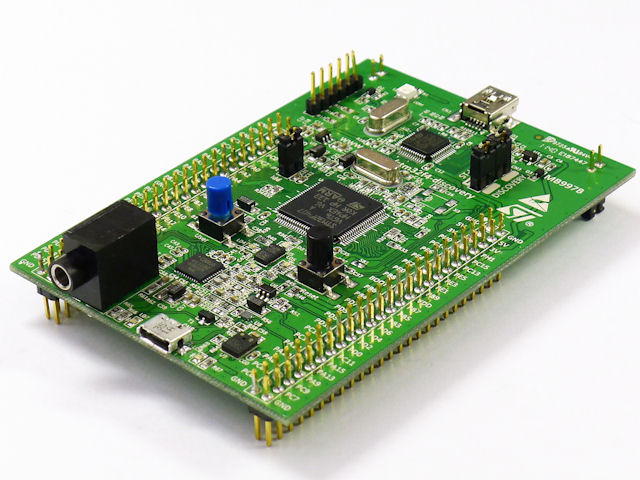
\includegraphics[height=8cm]{modulo_controle}
  \caption{Módulo de Controle}\label{fig:modulo_controle}
\end{figure}

O módulo de transmissão, responsável pela comunicação entre a inteligência e o módulo de controle do robô, consiste em uma placa comercial contendo o chip NRF24L01P e os periféricos necessários para o seu uso (ver Figura~\ref{fig:modulo_transmissao}). O módulo é ligado ao módulo de controle do robô através da placa mãe e se comunica com este utilizando o protocolo SPI (\textit{Serial Peripheral Interface}). Para fazer a comunicação com a inteligência, o módulo se comunica com outro igual ligado ao computador onde a inteligência está sendo executada utilizando uma frequência na faixa de 2,4 GHz. Para a comunicação entre dois módulos, o chip utiliza um protocolo próprio chamado Enhanced ShockBurst™, uma camada de vínculo de dados (camada de protocolo que lida com a entrada e saída de sequências de bits no meio físico, escondendo das camadas superiores o hardware subjacente e lidando com os pacotes perdidos e os pacotes duplicados) que permite envio de pacotes de confirmação sem a necessidade de receptor e transmissor inverterem seus modos de funcionamento (funcionalidade chamada \textit{Auto Acknowledgement}).
Isso permite ganhar tempo no envio das informações que a inteligência precisa.

\begin{figure}[H]
  \centering
  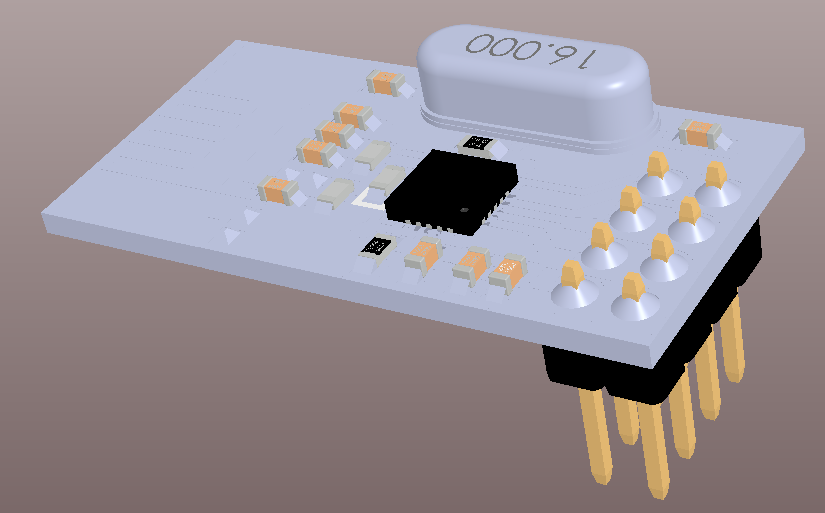
\includegraphics[height=8cm]{modulo_transmissao}
  \caption{Módulo de Transmissão}\label{fig:modulo_transmissao}
\end{figure}

Devido ao fato de o módulo de transmissão escolhido ser controlado por interface SPI, fez-se necessário aprender a utilizar a interface SPI do módulo de controle(STM32F4-Discovery), o que levou à confecção de uma  biblioteca de funções para comunicação SPI para o microcontrolador STM32F407VG.

% Ramificação constante ou taxa constante

% vim: tw=80 et ts=2 sw=2 sts=2 ft=tex spelllang=pt_br,en

%\chapter{Comunicação SPI}\label{cap:com_spi}

A interface periférica serial (SPI) permite comunicação serial half/ full-duplex, síncrona, com dispositivos externos. A interface pode ser configurada como mestre, caso em que fornece o sinal de relógio da comunicação (SCK) ao dispositivo externo escravo (\textit{slave}). A 
interface também é capaz de operar em configuração \textit{multimaster}.
Pode ser usada para uma variedade de propósitos, inclusive transferências síncronas simplex em duas linhas com uma possível linha de dados bidirecional ou comunicação confiável usando checagem CRC.
Normalmente, o SPI se conecta a dispositivos externos por 4 pinos:
\begin{itemize}
\item MISO: (\textit{Master In / Slave Out}) Esse pino é usado para transmitir dados do escravo para o mestre, no caso, do módulo de transmissão para o módulo de controle.
\item MOSI: (\textit{Master Out / Slave In}) Esse pino é usado para transmitir dados do mestre para o escravo, no caso, do módulo de controle para o módulo de transmissão.
\item SCK: (\textit{Serial Clock}) Esse pino é saída para o mestre e entrada para o escravo. É o sinal que determina a que instante os bits serão lidos
\item NSS: (\textit{Negated Slave Select}). Às vezes chamado de CSN, é um pino opcional para selecionar um dispositivo escravo, quando em nível baixo. Permite ao mestre do SPI comunicar-se com diversos escravos individualmente e evitar disputa pelas linhas de dados. Para este caso, foi usado um pino de um dos periféricos GPIO (\textit{General Purpose Input/Output} – Entrada/Saída de Propósito Geral) do módulo de controle, que foi configurado como saída.
\end{itemize}

Os pinos MOSI do mestre e do escravo são conectados, assim como os pinos MISO. Dessa forma, os dados são transferidos serialmente entre mestre e escravo (o bit mais significativo primeiro).
A comunicação é sempre iniciada pelo mestre. Quando o mestre transmite dados para um escravo através do pino MOSI, o escravo responde através do pino MISO. Isso implica uma comunicação full-duplex com dados de saída e de entrada sincronizados pelo mesmo sinal de relógio (provido pelo mestre através do pino SCK).
A Figura~\ref{fig:spi} ilustra o processo de comunicação com um mestre e um escravo.

\begin{figure}
	\centering
	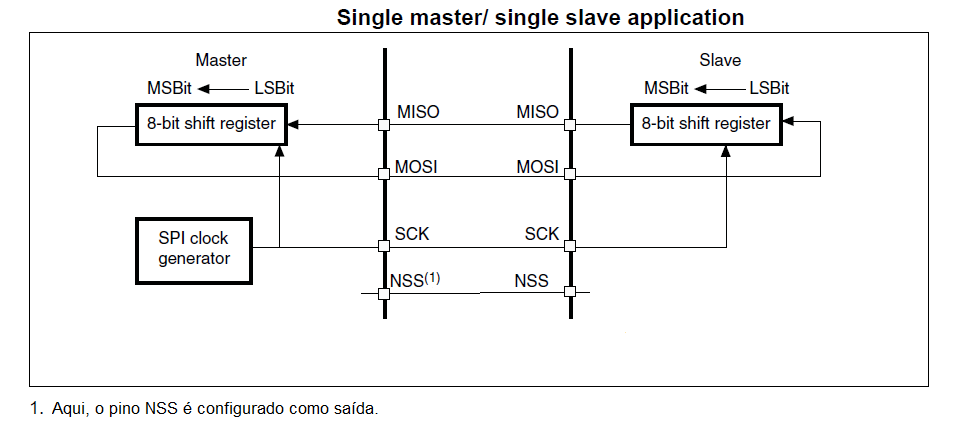
\includegraphics[scale=1]{SPI}
	\caption{Esquema da Comunicação SPI}
	\label{fig:spi}
\end{figure}

Para aprender a controlar a interface SPI do módulo de controle (mestre da comunicação), foram inicialmente feitos códigos em linguagem C, nos quais era feita a ativação do relógio do GPIO do pino NSS, configuração deste GPIO, a configuração dos registradores do periférico de SPI da Discovery e o envio de comandos para leitura de registradores do NRF24.
Após isso, foi feita a biblioteca, em C, para comunicação SPI para este microcontrolador, tendo sempre o manual de referência da STM como guia.

% Ramificação constante ou taxa constante

% vim: tw=80 et ts=2 sw=2 sts=2 ft=tex spelllang=pt_br,en

%\chapter{Necessidade da Abstração de Hardware}\label{cap:necessidade_abstr_hw}

O hardware do robô pode ser implementado de várias formas, por exemplo, com diferentes componentes e subsistemas, desde que suas funcionalidades básicas sejam preservadas e deseja-se que a maior parte do firmware seja independente das variações de implementações de hardware, característica chamada de modularidade. Para isso, cria-se uma camada de abstração entre os dispositivos físicos e a lógica que os comanda, cada módulo do robô é visto apenas como uma interface. Qualquer alteração feita na implementação de um módulo não tornará necessária a modificação de nenhuma outra parte do firmware, a menos que a interface tenha de ser modificada. Além disso, devido à SSL ser uma competição que almeja o avanço tecnológico na área de robótica, é interessante que o projeto possa continuar avançando independente das outras áreas, por isso quanto mais modular o trabalho, mais fácil se torna a realização de melhorias.

Os projetos da placa mãe, dos módulos de motor e do módulo de chute foram pensados com concepção modular justamente para que a abstração de hardware pudesse ser a mais abrangente possível. Ao fazer o módulo de chute e os módulos dos motores separados da placa mãe podemos modificá-los sem ter quer alterar nenhuma outra parte do projeto. O que precisa ser mantido é a funcionalidade. Por exemplo: contanto que os módulos de motor recebam as informações necessárias da placa mãe e enviem as certas para os motores, não importa como este módulo foi contruído. O mesmo vale para a placa de chute e para o módulo de comunicação.

Abaixo, está descrito como os componentes tiveram sua funcionalidade abstraída.
O robô tem dois chutes diferentes, o alto e o baixo. Dentro de cada opção, pode-se ainda determinar a intensidade do chute. Logo, para que ele funcione, basta enviar um sinal indicando qual o chute a ser usado e um número indicando a intensidade.
Para o drible, é necessário apenas que o motor gire numa direção específica a uma certa velocidade, logo, basta que se envie um sinal PWM (Pulse Width Modulation – modulação por largura de pulso). Da mesma forma que o drible, as rodas devem funcionar com sinal PWM, entretanto, o motor das rodas pode inverter seu sentido, portanto, são necessários dois sinais PWM, um para cada sentido. Para se enviar um sinal PWM são necessários o duty cycle e a frequência. Assumindo a frequência constante para todos os sinais, o PWM fica em função apenas do duty cycle. Como é utilizado um motor DC em cada roda, é necessário o uso de um encoder para se determinar sua velocidade de giro. Para tal, é preciso um contador de tempo, ou timer, e saber o número de divisões em uma volta completa do encoder. Sabendo o tempo transcorrido e a diferença entre os valores lidos, calcula-se a velocidade de giro do motor.
O conversor analógico digital, ou ADC (Analog to Digital Converter – conversor analógico para digital) lê uma tensão analógica e converte para uma representação digital. O funcionamento dos sensores depende da leitura de um sinal digital. No caso do sensor de presença da bola, que fica no drible, é enviado um pulso caso detecte algo.
A interface de SPI precisa apenas de funções para escrever um byte ou um buffer e funções para iniciar e terminar a transmissão. Como leitura e escrita ocorrem simultaneamente, para ler basta escrever algo e retornar o que o escravo enviou.
Quanto ao módulo de transmissão, basicamente, há as funções para transmitir pacotes e para verificar se há algum pacote recebido disponível para leitura.

Nota-se a interdependência entre os itens, por exemplo, tanto o motor das rodas como o drible utilizam sinais PWM, que por sua vez também está abstraído. Para utilizar sinais PWM para duas funções diferentes não é necessário alterar sua implementação.
Uma das aplicações disto no robô está no controle dos motores. Enquanto há camadas responsáveis por iniciar os encoders e os motores, há outra separada designada para usar os valores enviados por estas para realizar o controle de velocidades. Ressalta-se que nenhuma camada sabe o que acontece dentro da outra, sendo relevante para as demais somente o que elas recebem e enviam.

% Ramificação constante ou taxa constante

% vim: tw=80 et ts=2 sw=2 sts=2 ft=tex spelllang=pt_br,en

%\chapter{Biblioteca em C++}\label{cap:bibl_cpp}

Para a aplicação de abstração de \textit{hardware}, é necessária uma linguagem de programação que acompanhe suas condições de funcionamento, como poder relacionar diferentes objetos e fazer com que dependam de outros, podendo relacionar a funcionalidade e a implementação dos componentes do \textit{firmware}. Uma linguagem apropriada é C++, por ser orientada a objetos, podem-se criar classes para cada objeto desejado. C++ conta também com polimorfismo e herança de classes que são úteis para a abstração desejada. Por ser uma linguagem de alto desempenho e bem consagrada, há amplo suporte disponível para aprimoramento do código e resolução de possíveis problemas.
Assim, após a confecção da biblioteca SPI em C, foi feito um estudo da linguagem C++, usando diversas fontes, dentre elas:
\begin{itemize}
\item Paul Deitel, H. M. Deitel. How to program. Prentice Hall, 2005.
\item http://www.cplusplus.com/reference/
\item http://www.learncpp.com/
\end{itemize}

O antigo \textit{firmware} da RoboIME, em linguagem C e partes do \textit{firmware} (em C++) do rádio TPP-1400 da IMBEL, também foram valiosos para aprendizado da linguagem C++ e serviram de inspiração.

Em seguida, a biblioteca do SPI foi reescrita, incorporando códigos anteriores a uma hierarquia de classes composta pelas classes:
Quanto ao módulo de transmissão, ele corresponde a uma classe NRF24L01P que herda de uma classe abstrata MODEM (uma classe de interface), e possui em seu interior objetos da classe abstrata IO_PIN representando seus pinos, bem como um SPI_STM32 que representa a interface SPI com o módulo de controle, que por sua vez herda da classe abstrata SPI (outra classe de interface).

% Ramificação constante ou taxa constante

% vim: tw=80 et ts=2 sw=2 sts=2 ft=tex spelllang=pt_br,en

%\chapter{Desenho e Prototipagem das Placas Mãe, Placas de Chute e Placas Acionadoras dos Motores dos Robôs}\label{cap:design_placas}

O projeto das placas foi feito em duas etapas. A primeira etapa foi o desenvolvimento do esquemático do circuito, representação simbólica dos componentes e suas ligações. Nessa fase foram selecionados os componentes. A segunda etapa foi o \textit{layout}, em que foi feito um CAD (\textit{Computer Aided Design} ­– desenho assistido por computador) com o posicionamento dos componentes e o desenho das trilhas de cobre, tomando por base o esquemático. Foi preciso levar em conta a corrente que circularia pelo circuito para definir a larguras das trilhas, os tamanhos dos componentes a serem soldados e o tamanho da placa que seria produzida. Ao projetar as placas, os alunos da iniciativa adquirem experiência tanto em desenho de PCBs (\textit{Printed Circuit Board} – placa de circuito impresso), como em soldagem de componentes SMD (\textit{Surface Mounted Device} – dispositivo montado em superfície).

Para o desenvolvimento das placas, foi utilizado o \textit{software} \textit{Altium Designer\textsuperscript{\textregistered}}. As Figuras ~\ref{fig:blocos_placa_mae} apresentam os diagramas de blocos feitos a partir de esboços dos desenhos das três placas, utilizando uma das funcionalidades do \textit{Altium}.

Na placa mãe, o módulo de transmissão envia os dados recebidos da inteligência para o microcontrolador (que fica no módulo de controle adquirido) via protocolo SPI.
O módulo de controle envia sinais PWM para os módulos de motores e um pulso e um sinal digital para o módulo do chute. As correntes nos módulos de motores são medidas por circuitos integrados dedicados e enviadas para o módulo de controle via protocolo I2C.

Para funcionamento dos motores, são usados drivers e uma ponte H, para que os motores possam trabalhar nos dois sentidos.
Feito dessa forma, o \textit{hardware} passa a ter o fluxograma apresentado na Figura\ref{fig:func_hw}. Os comandos chegam através do módulo de comunicação e pela placa mãe é transmitida até a o módulo de controle (\textit{Discovery} STM32F4), que então a envia aos módulos pertinentes, motores ou chute. Há quatro motores ligados às rodas e um ao drible. O chute está separado em forte (baixo) e fraco (alto). Para fazer o controle das velocidades de giro de cada roda, informações sobre as rotações das rodas são passadas para a \textit{Discovery}, que pode também passá-las para o módulo de transmissão, se for o caso.

\begin{figure}
	\centering
	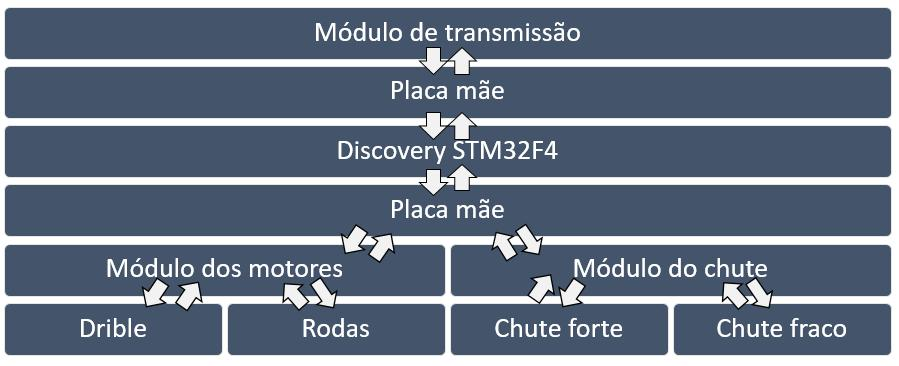
\includegraphics[scale=0.5]{funcionamento_hw}
	\caption{Funcionamento do \textit{hardware}}
	\label{fig:func_hw}
\end{figure}

%\begin{figure}
%	\centering
%	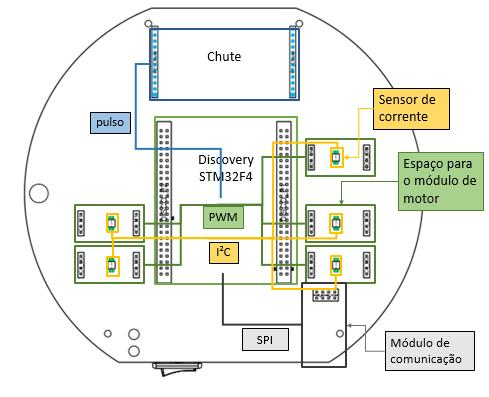
\includegraphics[scale=1]{blocos_placa_mae}
%	\caption{Diagrama de blocos da Placa Mãe}
%	\label{fig:blocos_placa_mae}
%\end{figure}

\section{Placa Mãe}\label{sec:placa_mae}

A placa-mãe (Figura~\ref{fig:modulo_placa_mae}) é responsável por fazer a ligação entre os atuadores do robô, transmitindo potência da bateria para os módulos de motor e de chute, fazendo a ligação entre esses módulos e os respectivos atuadores, fornecendo tensão aos circuitos lógicos e fazendo a ligação entre o módulo de controle e os sensores do robô -, no caso um sensor de quadratura em cada motor e o sensor ótico do chute que verifica a posse da bola. 

\begin{figure}
	\centering
	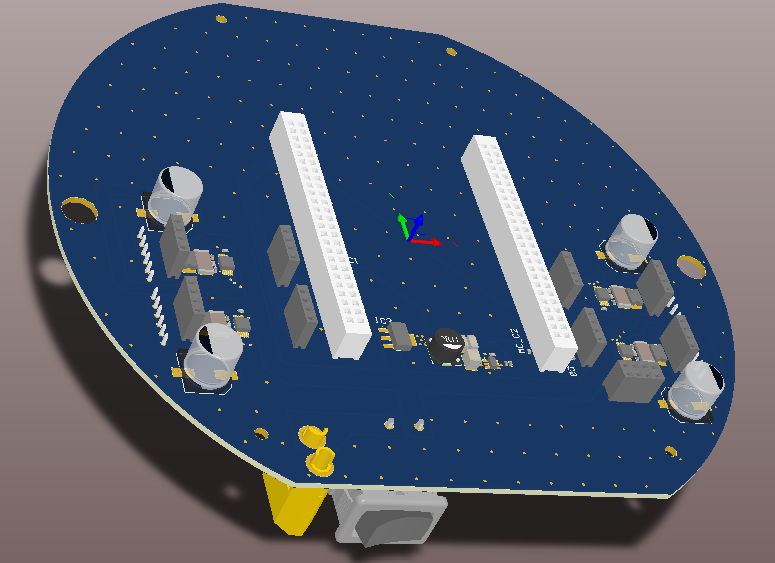
\includegraphics[scale=1]{modulo_placa_mae}
	\caption{Módulo da placa-mãe}
	\label{fig:modulo_placa_mae}
\end{figure}

\begin{figure}
	\centering
	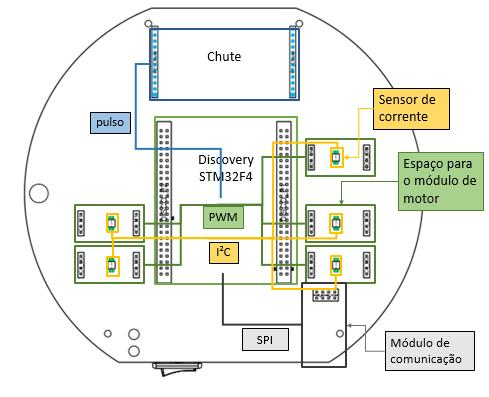
\includegraphics[scale=1]{blocos_placa_mae}
	\caption{Diagrama de blocos da placa mãe}
	\label{fig:blocos_placa_mae}
\end{figure}

Para que as conexões elétricas através da placa sejam feitas de modo seguro, a placa mãe contém um fusível, um capacitor de tanque, um capacitor de desacoplamento, e um sensor de corrente, o chip INA220, na entrada de cada módulo de motor e na entrada do módulo de chute, além de um circuito de divisão de tensão para que o módulo de controle seja capaz de controlar o nível de tensão da bateria.
O controle dessa placa é feito no firmware através da classe INA220, que faz a comunicação com os sensores de corrente na placa e a classe bateria que controla o nível da bateria sendo usada pelo robô. Essas classes permitem o controle dos circuitos de segurança do robô de maneira que o firmware possa lidar com comportamentos anômalos.
O desenho dessa placa foi reformulado:

\begin{itemize}
  \item As trilhas nos caminhos de potência foram trocados por planos para diminuir a resistência e o aquecimento das trilhas;
  \item Os antigos fusíveis simples foram trocados por fusíveis resetáveis para evitar que precisasse ser trocado durante a competição ou a 		cada sobrecorrente;
  \item Os antigos capacitores de tanque through hole foram trocados por capacitores SMD visando automatizar o processo de montagem utilizando 			uma pick and place automática;
  \item Os sensores de corrente também foram trocados por sua versão mais moderna e foi corrigido um erro no esquemático da placa mãe;
  \item O conector do módulo de transmissão foi trocado para ser compatível com o novo módulo de transmissão adotado pelo time.
\end{itemize}

% vim: tw=80 et ts=2 sw=2 sts=2 ft=tex spelllang=pt_br,en

\section{Módulo do Motor}\label{sec:modulo_motor}

Os módulos de motor (Figura~\ref{fig:modulo_motor}) fazem o controle dos quatro motores responsáveis pelo movimento do robô e do motor responsável pela atuação do driblador. Cada módulo consiste em uma ponte H capaz de controlar a velocidade de um motor de corrente contínua em duas direções. 

\begin{figure}
	\centering
	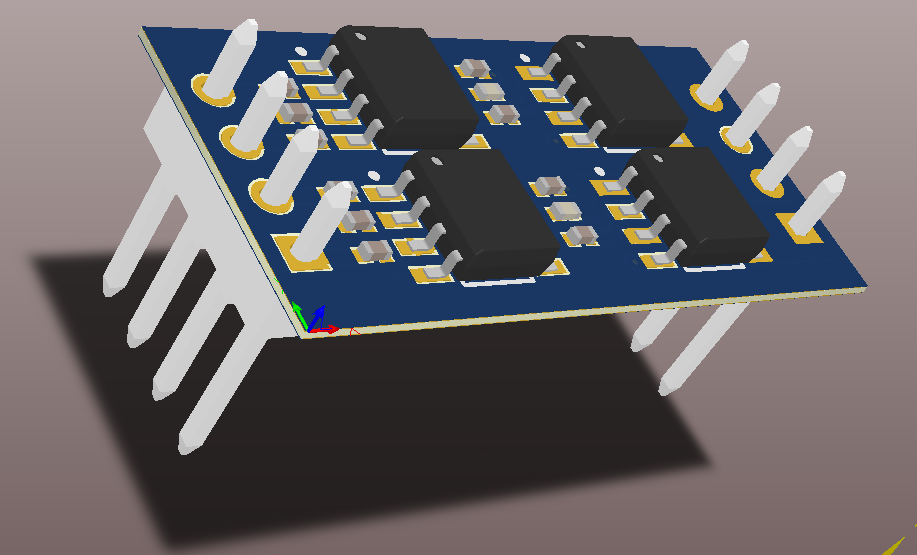
\includegraphics[scale=1]{modulo_motor}
	\caption{Módulo de Motor}
	\label{fig:modulo_motor}
\end{figure}

\begin{figure}
	\centering
	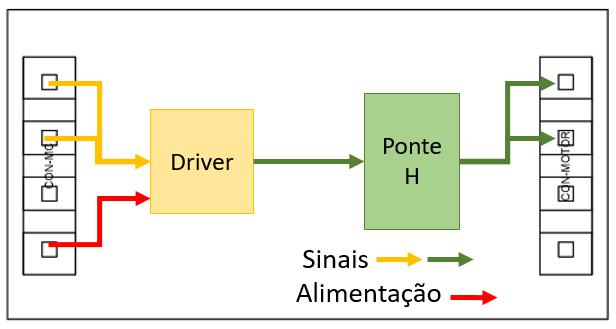
\includegraphics[scale=1]{blocos_motor}
	\caption{Diagrama de blocos do módulo de motor}
	\label{fig:blocos_motor}
\end{figure}

Esta placa é controlada pelo módulo de controle através da classe motor que utiliza a classe encoder para determinar a velocidade instantânea do motor. Com essa velocidade utiliza-se um algoritmo de controle PID para calcular a resposta que deve ser transmitida à placa, e envia-se essa resposta utilizando as classes degrau unitário e PWM.
O circuito de ponte H permite que o microcontrolador controle o sentido de rotação dos motores e a potência transmitida a eles, através do chaveamento dos transistores internos da ponte e amplificando o sinal enviado pelo microcontrolador.
O desenho dessa placa foi reformulado esse ano, as trilhas foram trocadas por planos nos caminhos de potência e foram adicionados um par de capacitores de desacoplamento na entrada dos drivers dos transistores.


% vim: tw=80 et ts=2 sw=2 sts=2 ft=tex spelllang=pt_br,en

\section{Módulo do Chute}\label{sec:modulo_chute}

O mecanismo de chute do robô foi elaborado utilizando dois solenóides como atuadores, um responsável pelo chute para frente e outro responsável pelo chute alto. E a placa (Figura~\ref{fig:modulo_chute}) é responsável por produzir a alta tensão necessária para ativar os dois solenóides, e transmitir a energia acumulada para acionar os atuadores.

\begin{figure}
	\centering
	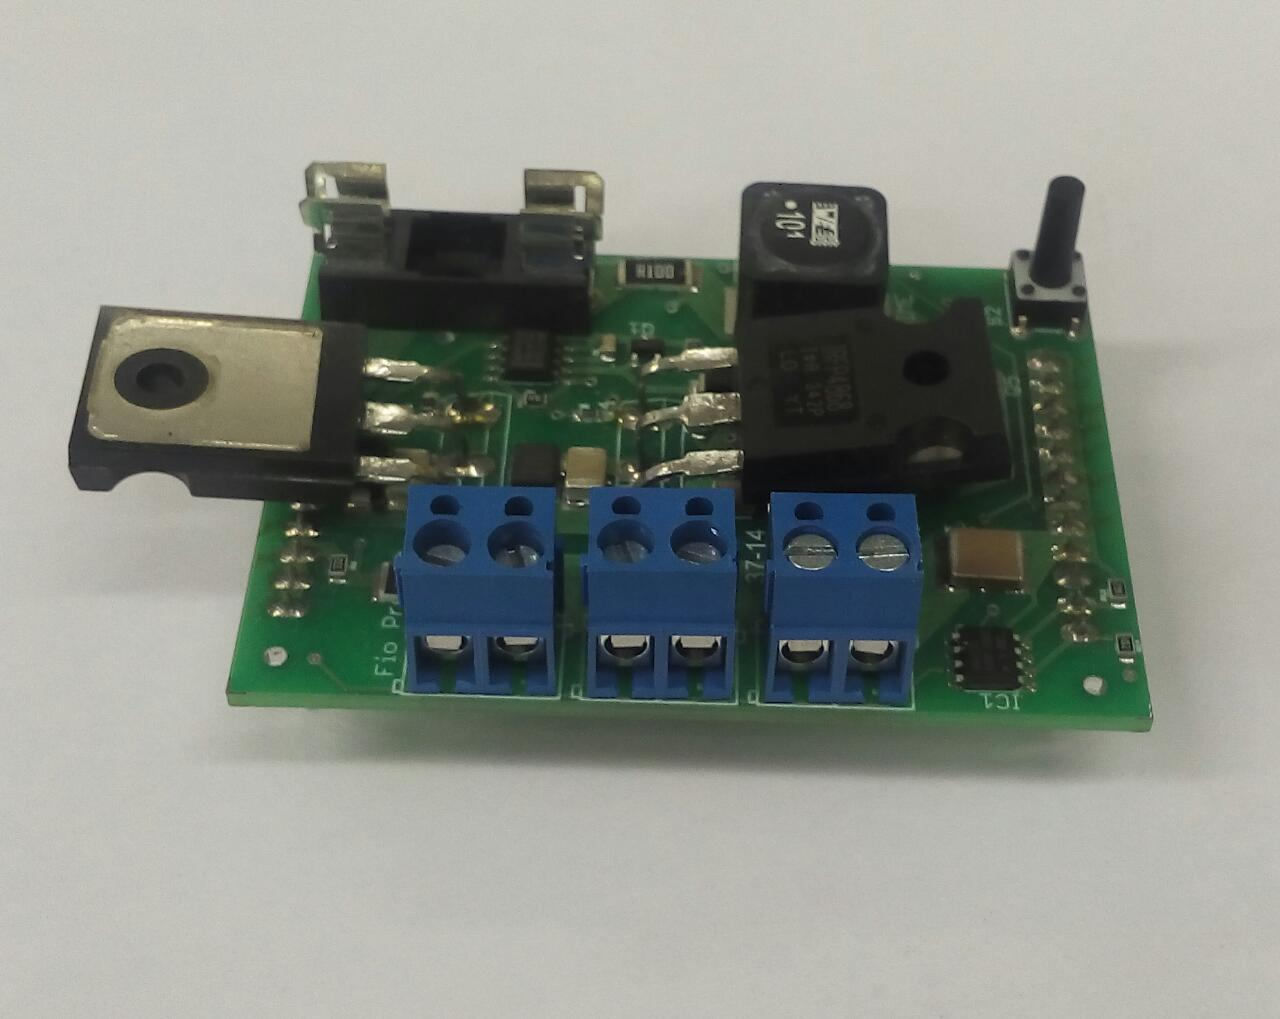
\includegraphics[scale=1]{modulo_chute}
	\caption{Módulo do Chute}
	\label{fig:modulo_chute}
\end{figure}

A placa funciona através de um circuito de conversão DC-DC controlado pelo circuito integrado MC34063 que converte os 7,8V DC da bateria em uma saída de 180V DC ligada a dois capacitores eletrolíticos de 2200 $\mu$F e 200V. Além desse circuito existe ainda um circuito para chavear a tensão dos capacitores nos solenóides, o que é feito utilizando um TC4427 driver de MOSFET e dois MOSFETs de potência IRFP4868PBF. 
O controle desse módulo é feito através da classe chute que utiliza a classe degrau unitário para limitar a energia transmitida a bola alterando a duração do intervalo de tempo que os MOSFETs ficarão ativados.

\begin{figure}
	\centering
	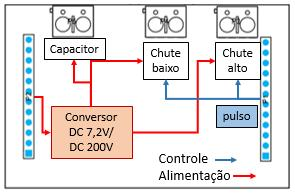
\includegraphics[scale=1]{blocos_chute}
	\caption{Diagrama de blocos do módulo de chute}
	\label{fig:blocos_chute}
\end{figure}


% vim: tw=80 et ts=2 sw=2 sts=2 ft=tex spelllang=pt_br,en


% Ramificação constante ou taxa constante

% vim: tw=80 et ts=2 sw=2 sts=2 ft=tex spelllang=pt_br,en

%\chapter{Participação na Competição Latin American Robotics Competition 2016}\label{cap:larc_2016}

A primeira versão do \textit{firmware} abstraído em \textit{hardware} foi completada a tempo da \textit{Latin American Robotics Competition} 2016 (LARC 2016), realizada em Recife, PE, em outubro de 2016. Os robôs, com novo \textit{firmware} e novas placas de circuito impresso, funcionaram como pretendido, sendo capazes de receber as informações da inteligência e executar os comandos. Entretanto, o projeto continuará evoluindo, pois aprimoramentos precisam ser feitos, por exemplo, nos controladores PID. Também pensa-se em trocar os motores DC por motores brushless. Fazer tais alterações será mais fácil, graças ao caráter modular do projeto.


% Ramificação constante ou taxa constante

% vim: tw=80 et ts=2 sw=2 sts=2 ft=tex spelllang=pt_br,en


% overview
No Capítulo~\ref{cap:overview}, uma visão geral do projeto físico do robôs é proposto.

% com_spi
No Capítulo~\ref{cap:com_spi}, é explicado o protocolo de comunicação utilizado pelo transmissor(responsável por receber comandos através de enlace de rádio) para se comunicar com o módulo controlador do robô.

% necessidade_abstr_h
No Capítulo~\ref{cap:necessidade_abstr_h}, são explicados os motivos que levaram à refatoração das bibliotecas de comunicação SPI e do módulo transmissor para adotar o conceito de abstração de \textit{hardware} e a linguagem C++. 

% bibl_cpp
No Capítulo~\ref{cap:bibl_cpp}, é falado sobre o processo de reescrita das referidas bibliotecas.

% design_placas
No Capítulo~\ref{cap:design_placas}, é falado sobre o processo de \textit{design} das novas placas de circuito impresso a serem usadas no projeto.

% larc_2016
No Capítulo~\ref{cap:larc_2016}, fala-se sobre a participação da RoboIME na \textit{Latin American Robotics Competition}(LARC).

% considerações finais
%No Capítulo~\ref{cap:cons_finais}, são apresentadas sugestões para trabalhos
%futuros e as principais dificuldades enfrentadas pelos autores são destacadas.

% conclusão
Finalmente, são apresentados os principais resultados atingidos neste trabalho.

% vim: tw=80 et ts=2 sw=2 sts=2 ft=tex spelllang=pt_br,en
